\documentclass[11pt,a4paper]{article}
\usepackage[margin=2.2cm]{geometry}
\usepackage{amsmath,amssymb,bm}
\usepackage{booktabs}
\usepackage{graphicx}
\usepackage{subcaption}
\usepackage{float}
\usepackage{tikz}
\usetikzlibrary{arrows.meta,positioning}
\usepackage[hidelinks]{hyperref}

\title{Comparison of Projected Heun/RK2 and Incremental Adams--Bashforth 2}
\author{Felix Scope}
\date{September 2026}

\begin{document}
\maketitle

\section{Purpose}

This private report compares the two implementations retained in the
repository. Both solve the same non-dimensional, axisymmetric incompressible
pipe-flow and heat-transfer problem on the same staggered finite-volume grid.
They use identical spatial operators, boundary conditions, physical
parameters, and convergence definitions. Only the temporal integration and
pressure-projection organization differ.

The production assignment report uses the Adams--Bashforth 2 implementation.
The Heun implementation is retained as an independent reference solution.

\section{Common discretization}

Both solvers use $n_r\times n_z=50\times250$, $\Delta r=0.01$,
$\Delta z=0.2$, $\Delta t=0.002$, $\mathrm{Re}=100$, and
$\mathrm{Pr}=5$. Convection is evaluated using second-order linear upwind
differencing and diffusion using second-order central differences. Pressure
and temperature are cell-centred; radial and axial velocity are stored on the
corresponding control-volume faces.

For both methods, a projection solves
\begin{equation}
 \nabla^2\phi=\frac{1}{\Delta t}\nabla\cdot\bm{u}^{*},
 \qquad
 \bm{u}^{\mathrm{new}}=\bm{u}^{*}-\Delta t\nabla\phi.
\end{equation}

\section{Projected Heun/RK2 method}

Let $F(\bm{u})$ contain the discrete convective and viscous momentum terms,
but not pressure. The Heun implementation performs
\begin{align}
 k_1 &= F(\bm{u}^{n}),\\
 \widehat{\bm{u}}_1 &= \bm{u}^{n}+\Delta t\,k_1,\\
 \bm{u}_1 &= \mathcal{P}(\widehat{\bm{u}}_1),\\
 k_2 &= F(\bm{u}_1),\\
 \widehat{\bm{u}}^{n+1}
 &=\bm{u}^{n}+\frac{\Delta t}{2}(k_1+k_2),\\
 \bm{u}^{n+1}&=\mathcal{P}(\widehat{\bm{u}}^{n+1}),
\end{align}
where $\mathcal{P}$ denotes the pressure projection. Projecting the
intermediate stage ensures that $k_2$ uses a divergence-free transport
velocity. This requires two momentum RHS evaluations and two Poisson solves
per complete step.

The old pressure is not included in the predictor. Consequently, the final
Poisson unknown is the complete non-incremental projection pressure rather
than a correction. The stored pressure is therefore blended toward it:
\begin{equation}
 p^{n+1}=(1-\alpha_p)p^n+\alpha_p\phi^{n+1}.
\end{equation}

Temperature is advanced with the same explicit trapezoidal weights and uses
the projected intermediate velocity in its second stage.

\section{Incremental Adams--Bashforth 2 method}

The AB2 method extrapolates the explicit RHS from two time levels:
\begin{equation}
 F^{AB2}=\frac{3}{2}F^n-\frac{1}{2}F^{n-1}.
\end{equation}
Because no previous RHS exists initially, the first step uses forward Euler.
Subsequent predictors include the known pressure gradient:
\begin{equation}
 \bm{u}^{*}=\bm{u}^{n}+\Delta t
 \left(F^{AB2}-\nabla p^n\right).
\end{equation}
One Poisson solve produces the pressure correction $p'$, after which
\begin{equation}
 \bm{u}^{n+1}=\bm{u}^{*}-\Delta t\nabla p',
 \qquad p^{n+1}=p^n+\alpha_p p'.
\end{equation}
Temperature uses AB2 on its convection--diffusion RHS. The method requires
one current RHS evaluation, stored previous RHS arrays, and one Poisson solve
per step.

\section{Direct comparison}

\begin{table}[H]
\centering
\caption{Algorithmic differences per complete time step.}
\begin{tabular}{p{4.4cm}p{4.5cm}p{4.5cm}}
\toprule
Property & Projected Heun/RK2 & Incremental AB2 \\
\midrule
Temporal form & two-stage, one-step & two-level, multistep \\
Formal temporal order & second & second after startup \\
Startup & self-starting & first-order Euler first step \\
Momentum RHS evaluations & two & one \\
Poisson solves & two & one \\
Stored previous RHS & not required & required \\
Old pressure in predictor & no & yes \\
Poisson unknown & full projection pressure & pressure correction \\
Pressure update & relaxed replacement & relaxed addition \\
\bottomrule
\end{tabular}
\end{table}

The AB2 formulation is less expensive per step because sparse pressure
solutions dominate the computational cost. Heun is self-starting and its
stage structure is often easier to generalize, but the correctly projected
version doubles the Poisson work. AB2 also corresponds directly to the
procedure recorded in the lecture notes.

\begin{figure}[H]
\centering
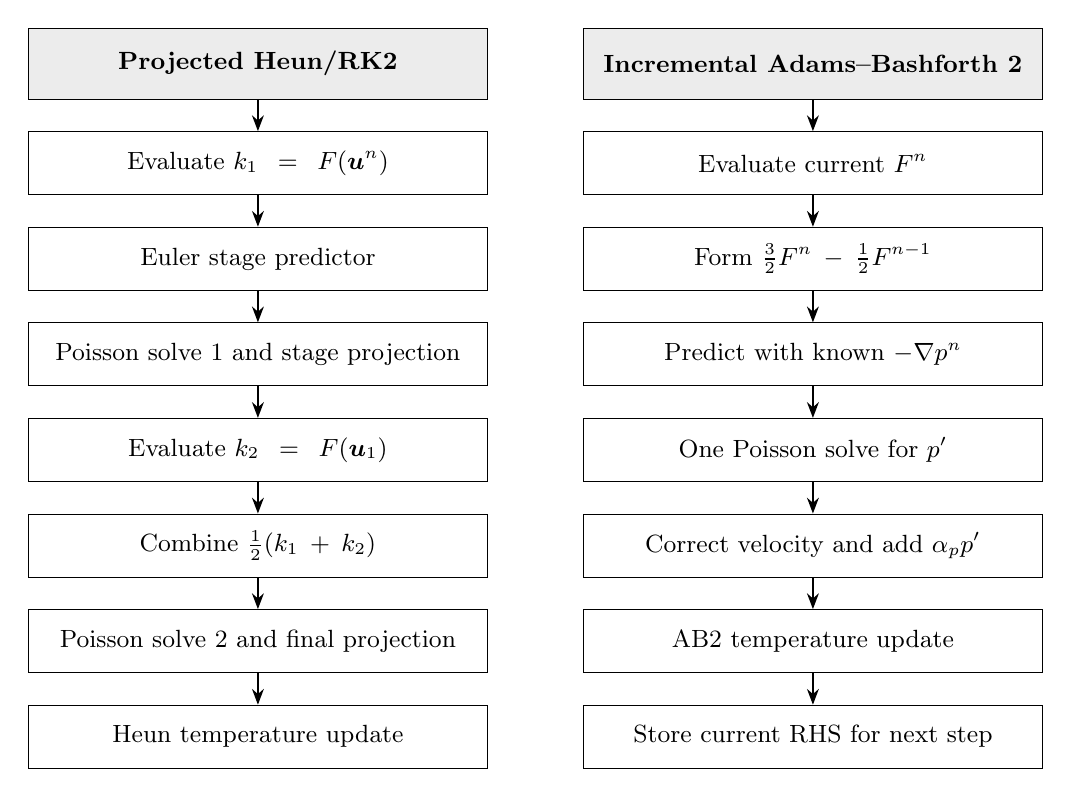
\begin{tikzpicture}[
  node distance=4mm,
  box/.style={rectangle, draw, align=center, text width=5.6cm,
              minimum height=8mm, font=\small},
  head/.style={rectangle, draw, fill=gray!15, align=center,
               text width=5.6cm, minimum height=9mm, font=\small\bfseries},
  arrow/.style={-{Stealth[length=2mm]}, thick}
]
\node[head] (hh) {Projected Heun/RK2};
\node[box, below=of hh] (h1) {Evaluate $k_1=F(\bm{u}^n)$};
\node[box, below=of h1] (h2) {Euler stage predictor};
\node[box, below=of h2] (h3) {Poisson solve 1 and stage projection};
\node[box, below=of h3] (h4) {Evaluate $k_2=F(\bm{u}_1)$};
\node[box, below=of h4] (h5) {Combine $\tfrac12(k_1+k_2)$};
\node[box, below=of h5] (h6) {Poisson solve 2 and final projection};
\node[box, below=of h6] (h7) {Heun temperature update};

\node[head, right=12mm of hh] (ah) {Incremental Adams--Bashforth 2};
\node[box, below=of ah] (a1) {Evaluate current $F^n$};
\node[box, below=of a1] (a2) {Form $\tfrac32F^n-\tfrac12F^{n-1}$};
\node[box, below=of a2] (a3) {Predict with known $-\nabla p^n$};
\node[box, below=of a3] (a4) {One Poisson solve for $p'$};
\node[box, below=of a4] (a5) {Correct velocity and add $\alpha_p p'$};
\node[box, below=of a5] (a6) {AB2 temperature update};
\node[box, below=of a6] (a7) {Store current RHS for next step};

\foreach \a/\b in {hh/h1,h1/h2,h2/h3,h3/h4,h4/h5,h5/h6,h6/h7,
                     ah/a1,a1/a2,a2/a3,a3/a4,a4/a5,a5/a6,a6/a7}
  \draw[arrow] (\a) -- (\b);
\end{tikzpicture}
\caption{Per-step workflows. The first AB2 step substitutes forward Euler
for the unavailable two-level extrapolation.}
\label{fig:method-flowchart}
\end{figure}

\section{Measured results}

Both implementations were run to 30,000 steps, corresponding to $t^*=60$.
The AB2 results were independently generated in Python and MATLAB. The final
reported residuals were
\begin{table}[H]
\centering
\begin{tabular}{lccc}
\toprule
Run & $R_{\mathrm{cont}}$ & $R_{\mathrm{vel}}$ & $R_T$ \\
\midrule
AB2, MATLAB & $6.43\times10^{-15}$ & $2.78\times10^{-14}$ & $2.19$ \\
AB2, Python & $1.30\times10^{-9}$ & $5.55\times10^{-14}$ & $2.19$ \\
Heun reference & $\mathcal{O}(10^{-13})$ & $\mathcal{O}(10^{-13})$ & $2.19$ \\
\bottomrule
\end{tabular}
\end{table}

The different continuity floors in the two AB2 programs arise from numerical
linear-solve precision and remain far below the required $10^{-6}$ tolerance.
Velocity is converged in both methods. Temperature is not temporally converged
at $t^*=60$ in either method. Its identical residual of $2.19$ demonstrates
that changing from Heun to AB2 does not remove the slow physical thermal
relaxation timescale.

\begin{figure}[H]
\centering
\begin{subfigure}[t]{0.49\textwidth}
 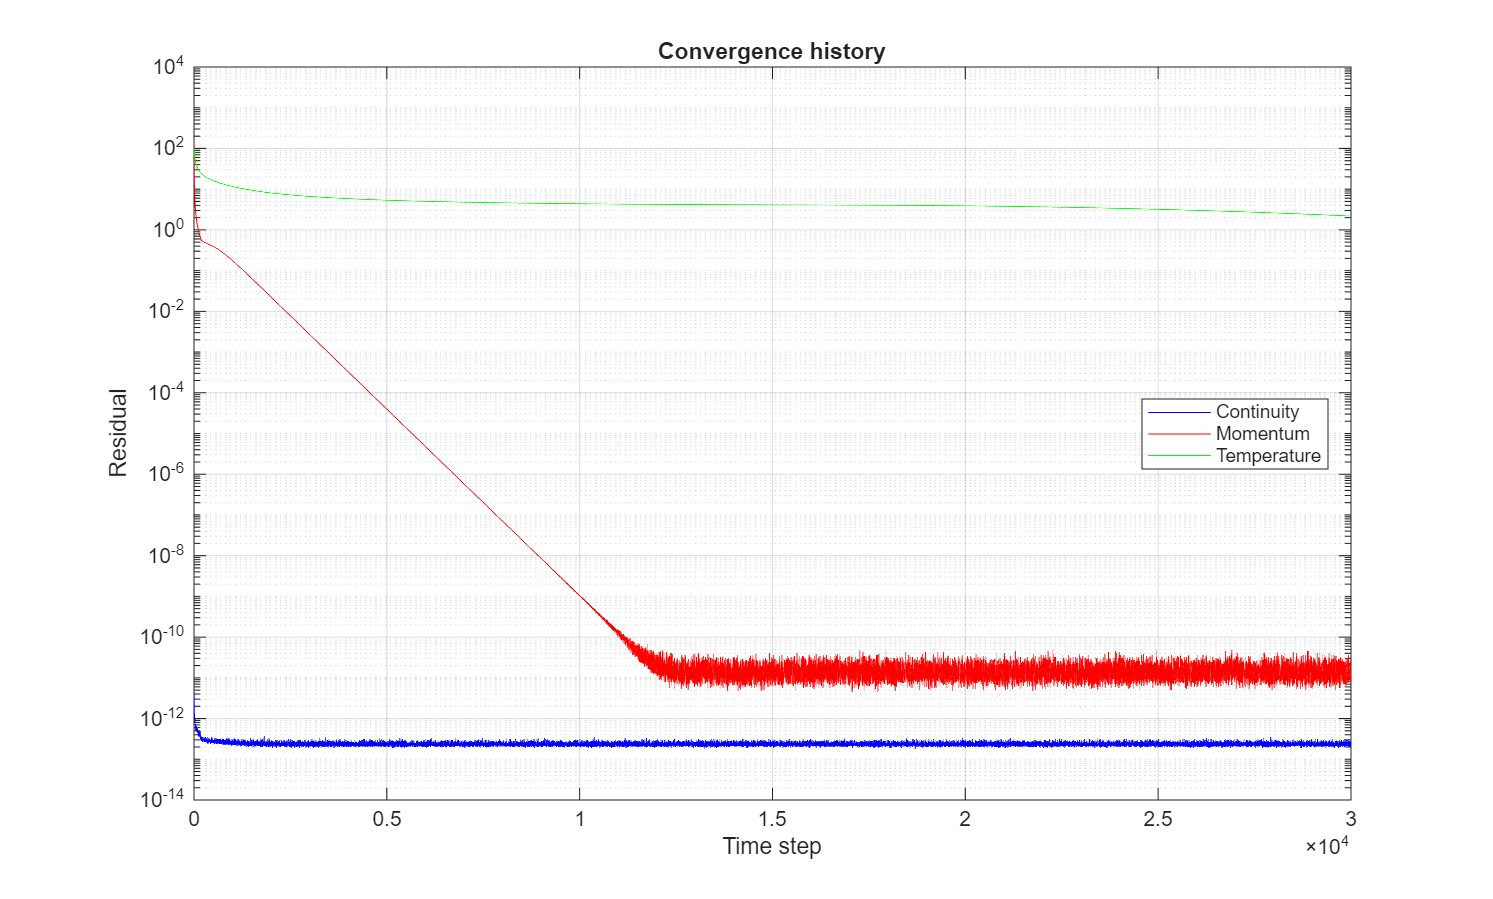
\includegraphics[width=\linewidth]{../Heun/Plots_matlab/convergence.png}
 \caption{Projected Heun/RK2.}
\end{subfigure}
\hfill
\begin{subfigure}[t]{0.49\textwidth}
 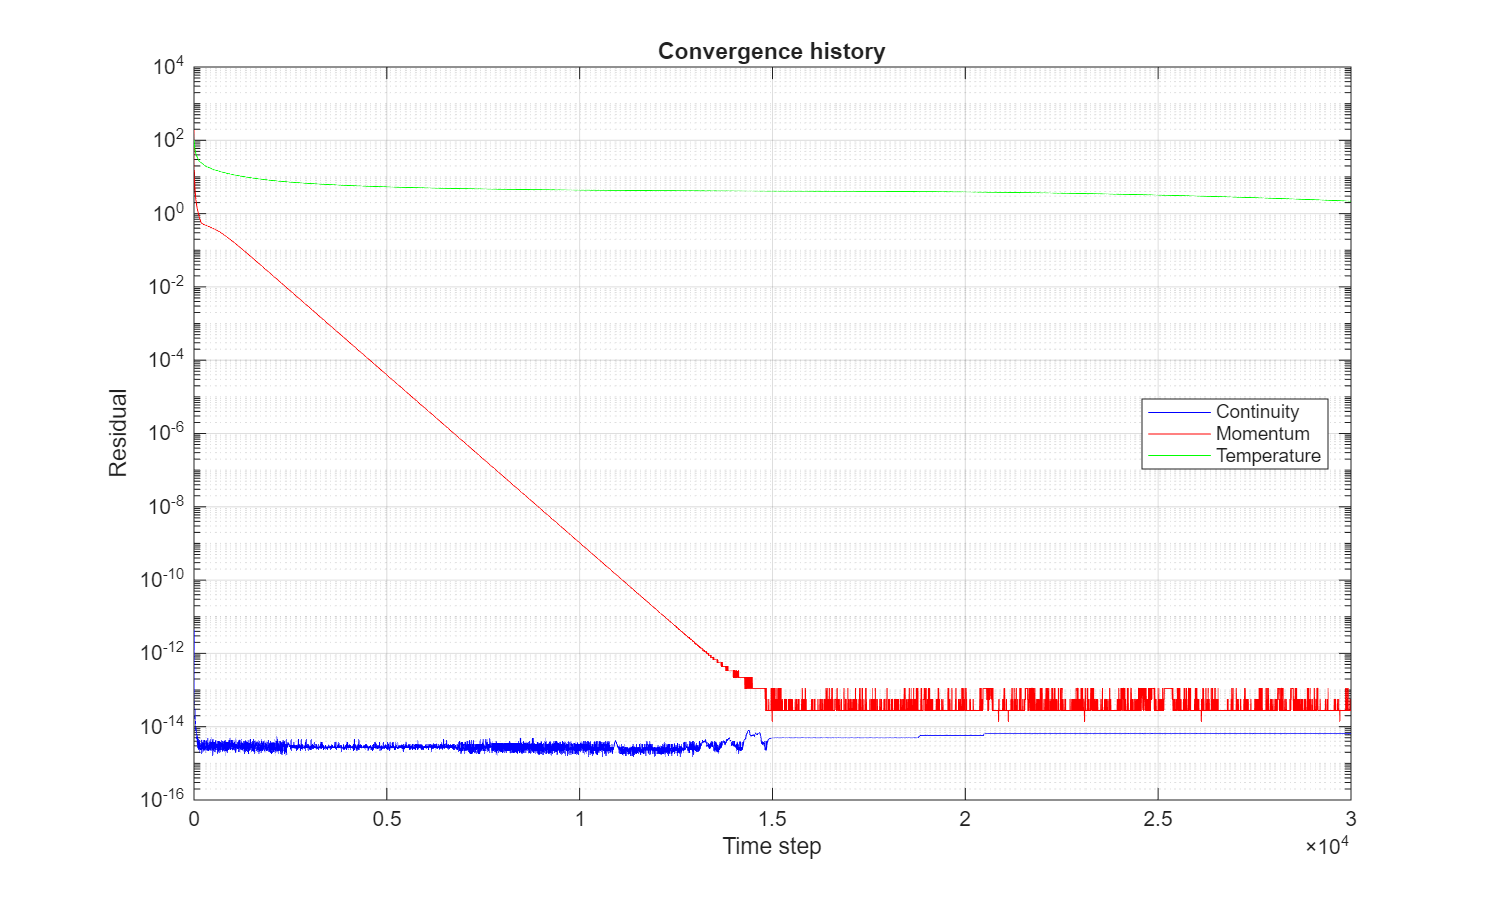
\includegraphics[width=\linewidth]{../AdamsBashfort2/Plots_matlab/convergence.png}
 \caption{Incremental AB2.}
\end{subfigure}
\caption{Convergence histories under identical physical and grid settings.}
\end{figure}

\begin{figure}[H]
\centering
\begin{subfigure}[t]{0.49\textwidth}
 \includegraphics[width=\linewidth]{../Heun/Plots_matlab/w_comparison.png}
 \caption{Projected Heun/RK2.}
\end{subfigure}
\hfill
\begin{subfigure}[t]{0.49\textwidth}
 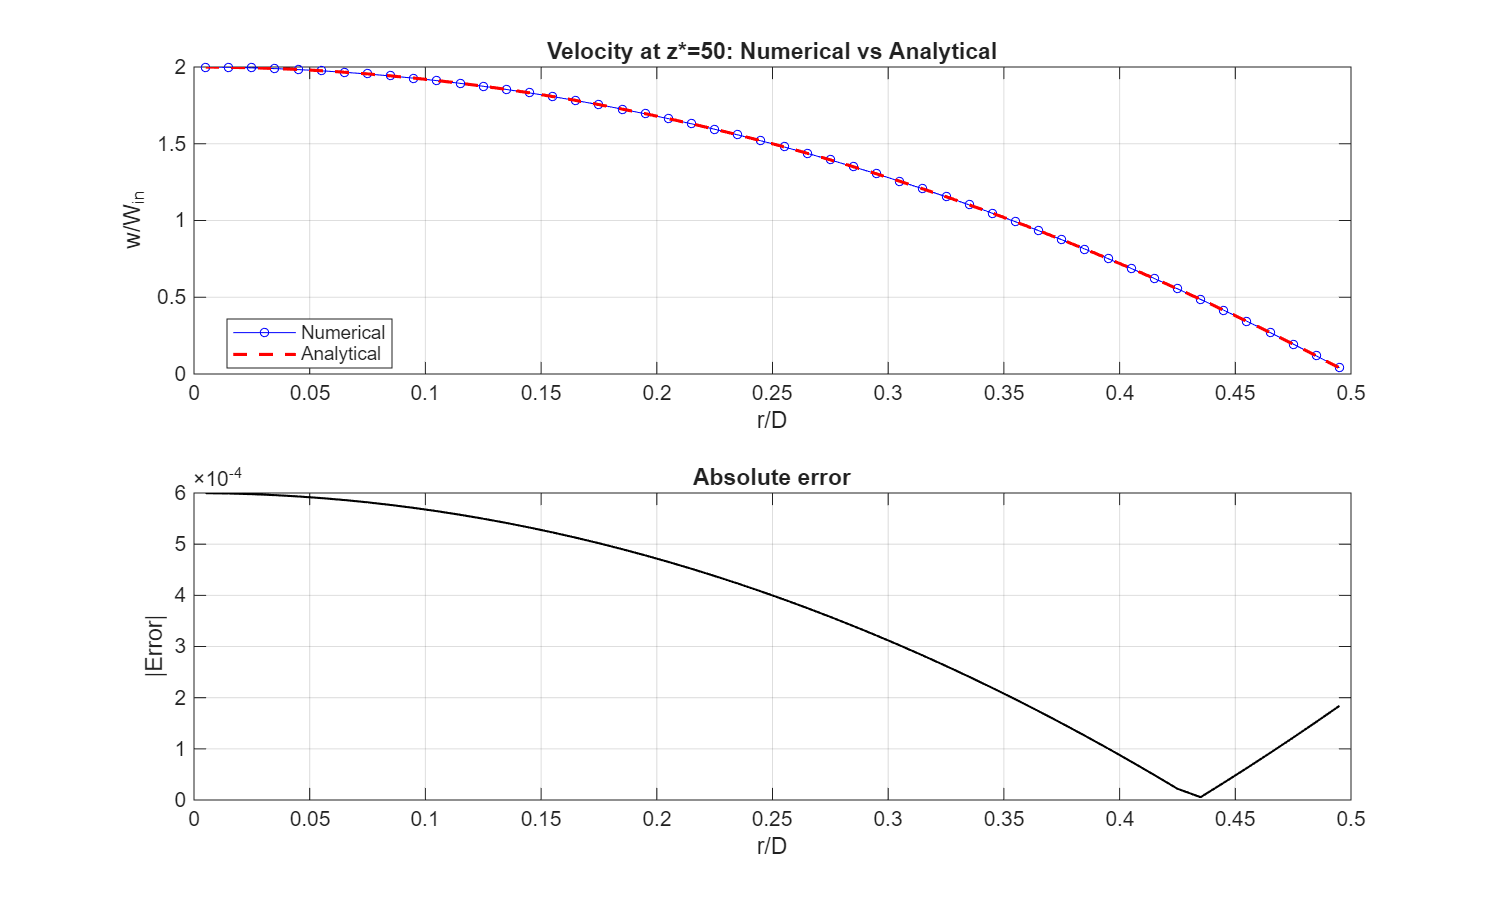
\includegraphics[width=\linewidth]{../AdamsBashfort2/Plots_matlab/w_comparison.png}
 \caption{Incremental AB2.}
\end{subfigure}
\caption{Fully developed axial velocity compared with Hagen--Poiseuille flow.}
\end{figure}

The two panels above are visually identical because both methods have reached
the same discrete steady momentum solution. Time integration determines the
transient path to that fixed point, but it does not change the converged
finite-volume equations. With velocity residuals near machine precision, the
remaining differences are below the plotted line width. Profiles saved at an
early common time would be a more sensitive comparison of temporal behavior.

\begin{figure}[H]
\centering
\begin{subfigure}[t]{0.49\textwidth}
 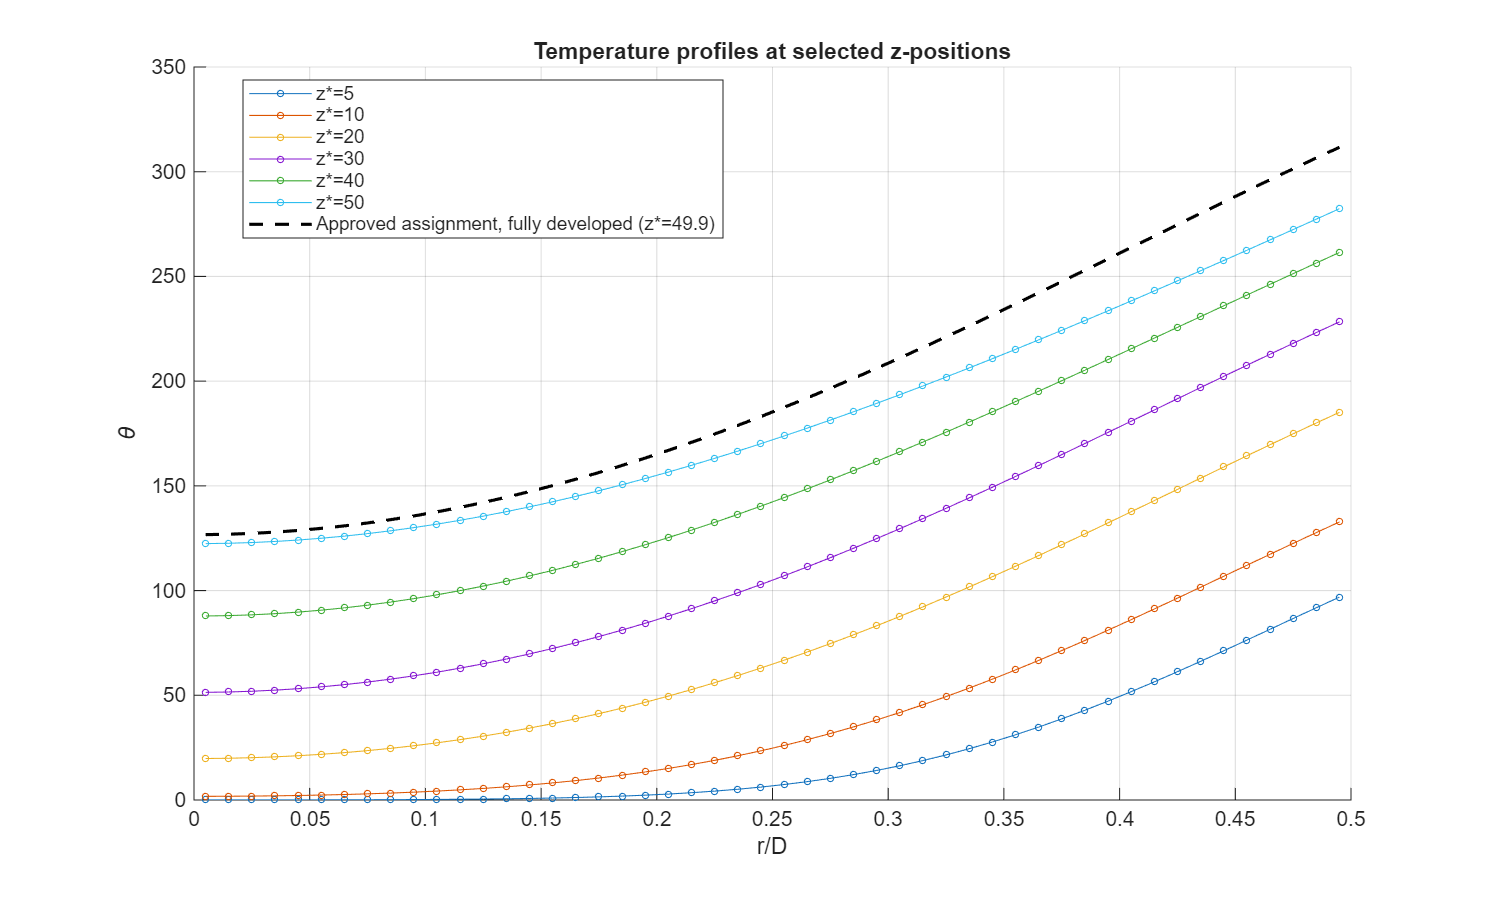
\includegraphics[width=\linewidth]{../Heun/Plots_matlab/T_profiles.png}
 \caption{Projected Heun/RK2.}
\end{subfigure}
\hfill
\begin{subfigure}[t]{0.49\textwidth}
 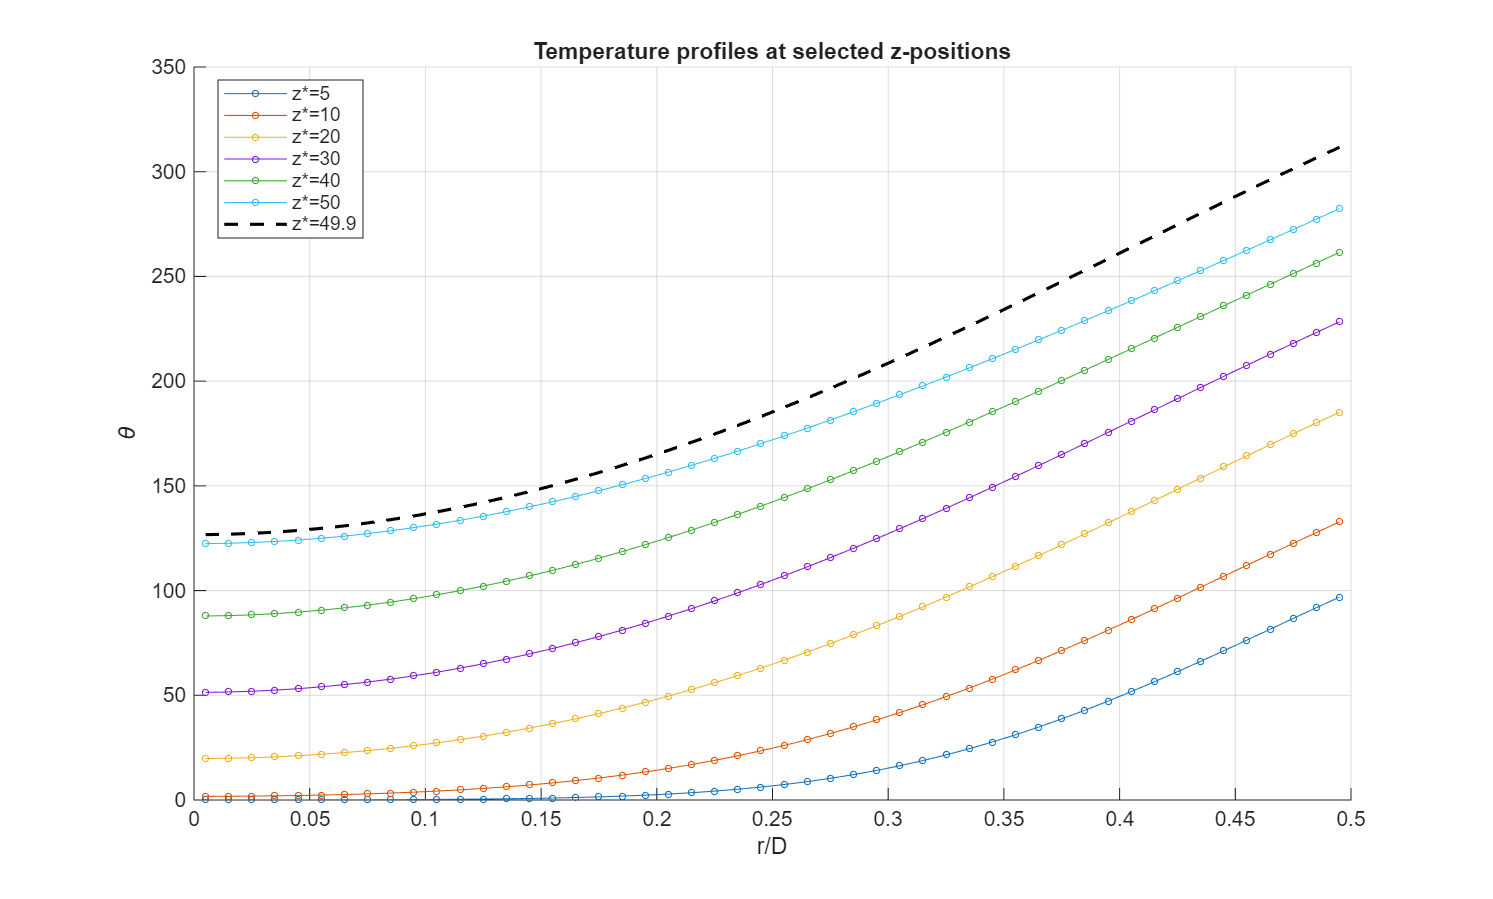
\includegraphics[width=\linewidth]{../AdamsBashfort2/Plots_matlab/T_profiles.png}
 \caption{Incremental AB2.}
\end{subfigure}
\caption{Temperature profiles after 30,000 time steps.}
\end{figure}

\section{Conclusion}

For this steady laminar test case, both second-order methods produce the same
engineering conclusions and effectively identical convergence behavior. AB2
is preferable for the assignment because it follows the documented lecture
algorithm and halves the number of Poisson solves per step. The Heun solver
remains useful as an independent cross-check. Neither method accelerates the
physical approach of the temperature field to steady state; longer simulated
time or a steady/implicit thermal treatment would be required for that.

\end{document}
